\documentclass{beamer}

% Russian-specific packages
\usepackage[T2A]{fontenc} % поддержка специальных русских символов
\usepackage[english,russian]{babel}
\usepackage[utf8]{inputenc}

% русские переносы
\usepackage{hyphenat}
% \hyphenation{ма-те-ма-ти-ка вос-ста-нав-ли-вать}

% путь к папке с изображениями
\graphicspath{{./figs/}}

% выравнивание по центру подписей к картинкам
\usepackage[justification=centering]{caption}

% Стиль презентации
\usetheme{Warsaw}
\usecolortheme{crane}
% Стиль цитирования
\bibliographystyle{utf8gost71u}

% Переопределение настроек цитирование на схожие с article
\usepackage[numbers]{natbib}
% make bibliography entries smaller
\renewcommand\bibfont{\scriptsize}
% If you have more than one page of references, you want to tell beamer
% to put the continuation section label from the second slide onwards
\setbeamertemplate{frametitle continuation}[from second]
% Now get rid of all the colours
\setbeamercolor*{bibliography entry title}{fg=black}
\setbeamercolor*{bibliography entry author}{fg=black}
\setbeamercolor*{bibliography entry location}{fg=black}
\setbeamercolor*{bibliography entry note}{fg=black}
% and kill the abominable icon
\setbeamertemplate{bibliography item}{}

% Замена стандартного (Cont.) на русский язык
\setbeamertemplate{frametitle continuation}[from second][(продолжение)]

% Убрать из подписи картинки префикс Рис.
\usepackage{caption}
\captionsetup[figure]{labelformat=empty}

\begin{document}

% Оформление титульного листа
\title[Развитие ППРЭ]
{Развитие метода разностной эволюции
для поиска параметров математических моделей}
\author[Свичкарев Анатолий]
{Студент: \textbf{Свичкарев Анатолий, группа 53601/4}\\
Научный руководитель: \textbf{Козлов Константин Николаевич}}
\institute[СПбПУ]
{Санкт-Петербургский Государственный
Политехнический Университет\\Петра Великого}
\date{март, 2016}

% Создание заглавной страницы
\frame{\titlepage} 

\begin{frame}{Введение}
Проведение вычислительного эксперимента
с помощью \textbf{математической модели}
в большинстве случаев обходится \textbf{значительно дешевле},
чем проведение соответствующего эксперимента
над реальным биологическим объектом,
кроме того \textbf{некоторые условия
невозможно воспроизвести в лаборатории}.
\bigskip

Математические модели в биоинформатике в
большинстве случаев создаются в таких компьютерных
системах расчетов как \textbf{R, Python, Octave} и др.
\bigskip

Нахождение параметров в таких моделях требует
многократного вычисления решений, что влечет
\textbf{большие накладные расходы} на запуск того или иного
интерпретатора.
\end{frame}

\begin{frame}{Цель}
\textbf{Развитие метода ППРЭ}

\bigskip
За счет единовременной загрузки
неизменяемых данных и
асинхронной загрузки переменных параметров
планируется достигнуть
\textbf{сокращения времени вычисления}
при использовании
интерпретируемых языков, например,
для системы статистических расчетов R.
\end{frame}

\begin{frame}{Задачи}
\begin{enumerate}
    \itemsep 2em
    \item реализовать расширение программы ППРЭ,
        позволяющее запускать нужное количество копий
        интерпретатора один раз при старте.
    \item провести численные эксперименты с тестовыми функциями
    \item провести сравнительный анализ полученных результатов
\end{enumerate}
\end{frame}

\begin{frame}{Разностная эволюция}
    \begin{block}{Разностная эволюция}
        --- стохастический итерационный алгоритм минимизации,
        предложенный Сторном и Прайсом в 1995 г.
    \end{block}
    \begin{figure}[!h]
        \centering
        % TODO максимальный доступный размер
        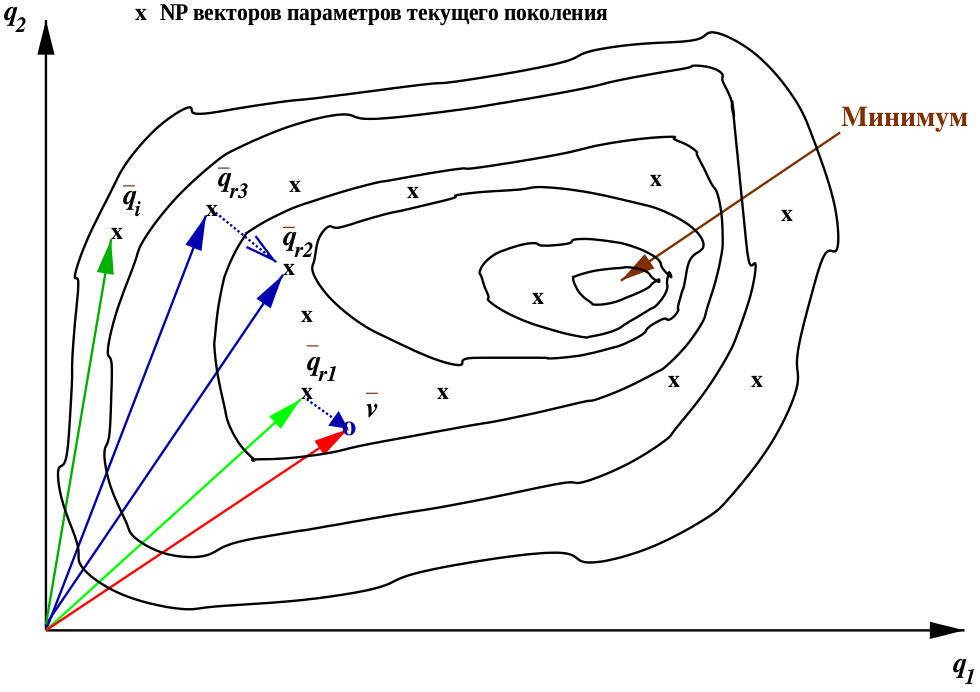
\includegraphics[scale=0.2]{DE}
        \caption{Геометрическая интерпретация метода разностной эволюции}
    \end{figure}
\end{frame}

\begin{frame}{Полностью параллельная разностная эволюция}
    \begin{block}{Полностью параллельная разностная эволюция (ППРЭ, DEEP)}
        --- эффективный метод решения
        обратной задачи математического моделирования,
        модификация глобального стохастического метода.
    \end{block}
    \bigskip

    Две модификации разностной эволюции,
    реализованные в DEEP:
    \bigskip

    \begin{itemize}
        \itemsep 1em
        \item Скрещивание с учётом значения функционала;
        \item Скрещивание для поддержания разнообразия индивидов.
    \end{itemize}
\end{frame}

\begin{frame}{Улучшение взаимодействия. Суть задачи.}
    \large{\textbf{Старая реализация:}}\\
    Для вычисления функционала
    качества каждый раз запускался
    новый экземпляр интерпретатора.
    \bigskip

    \large{\textbf{Новая реализация:}}\\
    Создаётся \textbf{пул потоков},
    где в каждом потоке запускается интерпретатор
    и инициализируется функцией из скрипта.\\
    Создаётся \textbf{асинхронная очередь задач},
    задачей является вектор индивида.\\
    Свободный интерпретатор из пула
    выбирает индивида и вычисляет на нём значение функционала.
    \textbf{Интерпретаторы не перезапускаются},
    а обрабатывают следующие задачи.
    \bigskip

    Используются структуры и алгоритмы
    кроссплатформенной библиотеки \textbf{GLib}.
\end{frame}

\begin{frame}{Методика экспериментов}
    \begin{figure}
        \makebox[\textwidth]{
            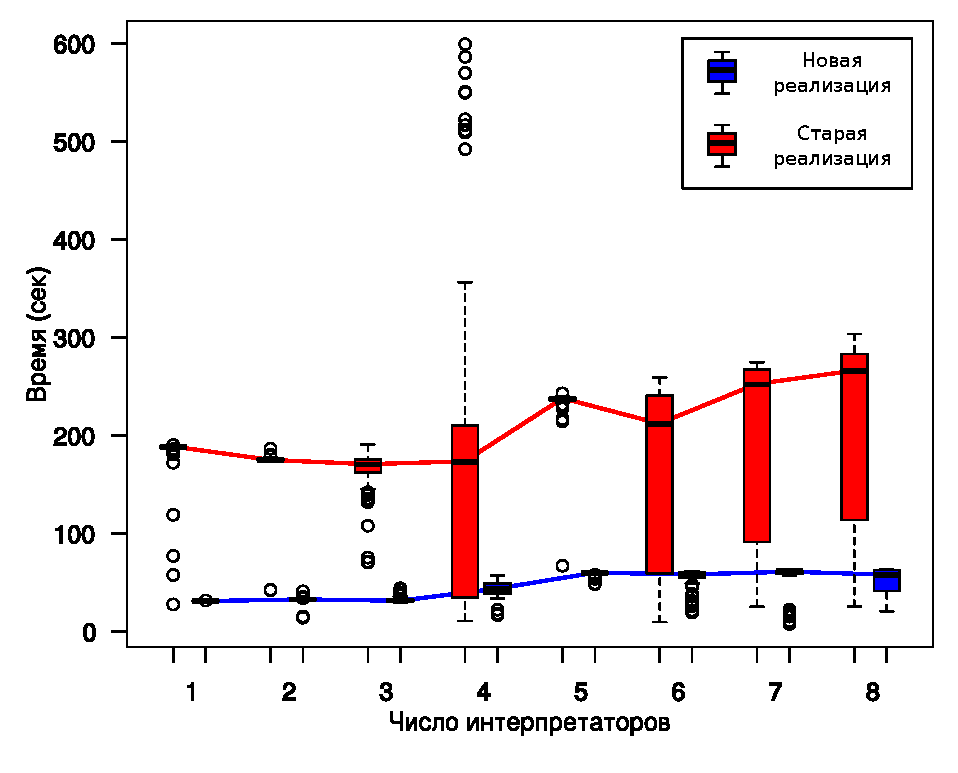
\includegraphics[width=0.5\paperwidth]{m5}
            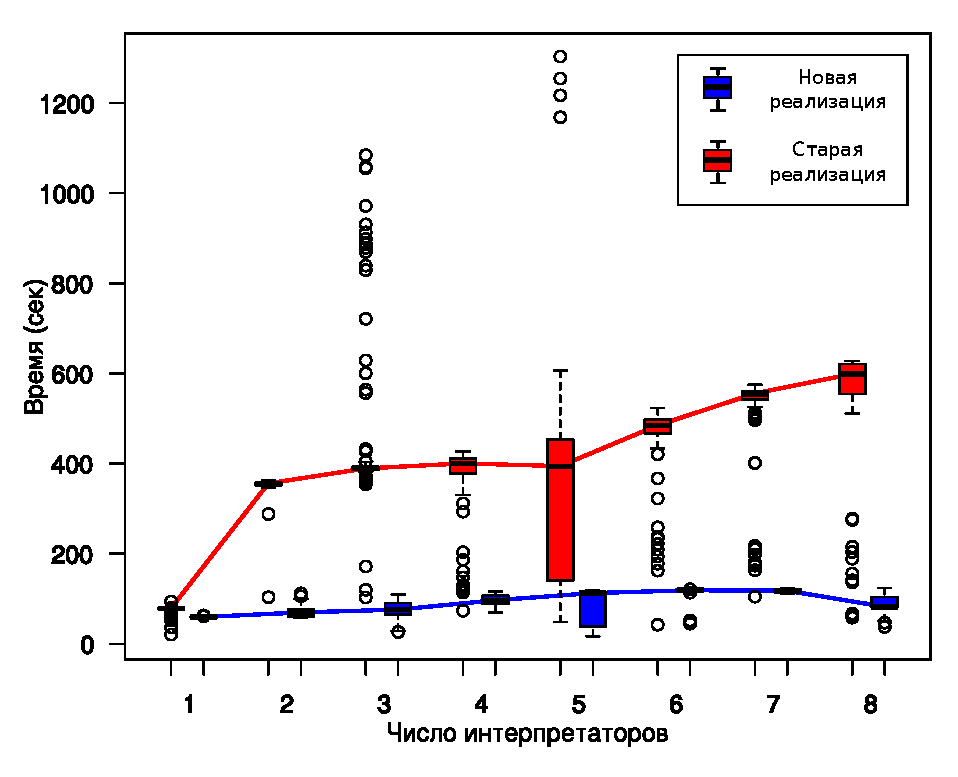
\includegraphics[width=0.5\paperwidth]{m10}
        }
        \caption{Медиана и полтора межквартильных расстояния
            времени выполнения при коэффициенте размера популяции
            5 и 10 соответственно}
    \end{figure}
\end{frame}

\begin{frame}{Статистическая обработка}
    График 95\% доверительных интервалов по критерию Тьюки.
    \begin{columns}
        \begin{column}{0.7\textwidth}
            \begin{figure}[!h]
                \centering
                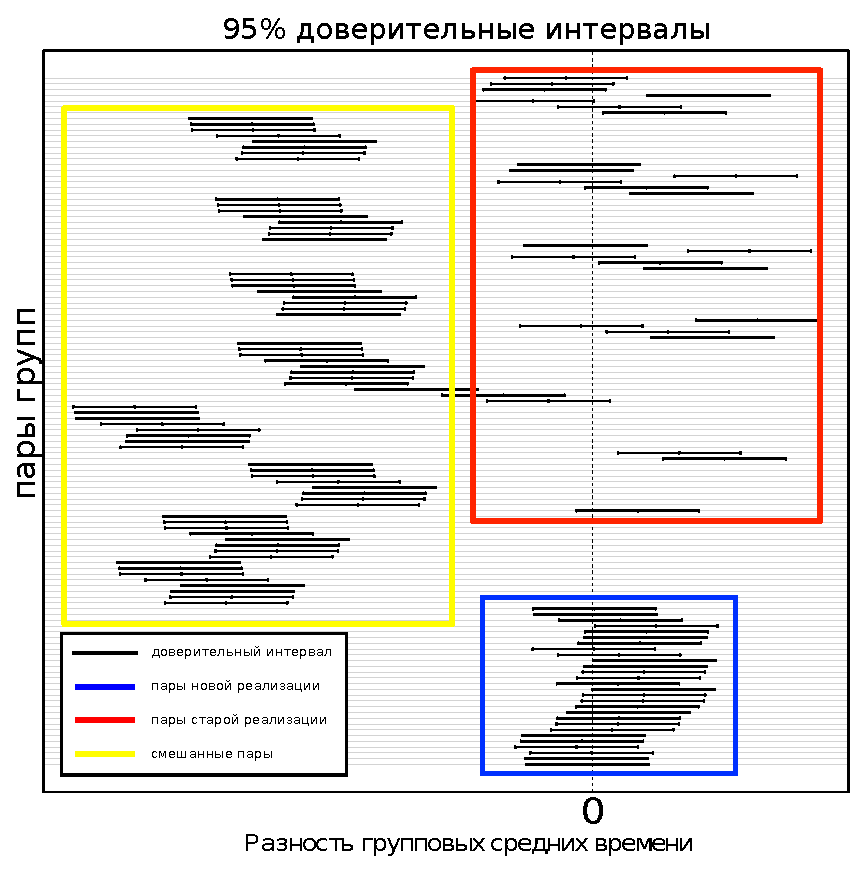
\includegraphics[width=.8\textheight]{tukey}
            \end{figure}
        \end{column}
        \begin{column}{0.4\textwidth}
            \textbf{\textcolor{red}{Красной рамка:}}\\
                старая реализация,
                конкуренция интерпретаторов
                за ресурсы при инициализации;

            \textbf{\textcolor{blue}{Синяя рамка:}}\\
                новая реализация, единичная инициализация;

            \textbf{\textcolor{yellow}{Жёлтая рамка:}}\\
                пары из старой и новой реализаций,
                оптимизация статистически значима.
        \end{column}
    \end{columns}
\end{frame}

\begin{frame}{Выводы}
\begin{itemize}
    \itemsep 2em
    \item Разработанный механизм обеспечивает
        \textbf{4x прирост производительности}
        на 4 параллельных потоках с 4 интерпретаторами по
        сравнению со старой реализацией;
    \item Разработанный механизм \textbf{сохраняет кроссплатформенность} DEEP
        (использовалась кроссплатформенная GLib).
\end{itemize}
\end{frame}

\begin{frame}{Благодарности}
    \begin{itemize}
        \itemsep 2em
        \item \textbf{Марии Георгиевне Самсоновой}
        \item \textbf{Константину Николаевичу Козлову}
        \item \textbf{Андрею Сергеевичу Писареву}
    \end{itemize}
    \bigskip

    \vfill
    \begin{center}
        \LARGE Спасибо за внимание!
    \end{center}
\end{frame}

% если не хватит слайда - продолжит на следующих
% t - пытается равномерно распределить
\begin{frame}[t,allowframebreaks]{Используемая литература}
    \nocite{Kozlov11, Kozlov13, Storn95, pisarev2015tracker,
    GLib, zaharie2002parameter, fan2003trigonometric}
    \bibliography{citations}
\end{frame}

\end{document}

